\documentclass{assignment}

\course{ECO 120-04}
\name{Lucas Reddinger}
\date{Monday 31 October 2022}
\doctitle{Assignment 7: Unemployment}

\begin{document}
\RaggedRight

\beginassignment{}

\emph{Due Friday 4 November.} Please submit hardcopy at the beginning of class (11:00 a.m.), or if you prefer, under the door of Wimberly Hall 339C by 10:50 a.m.

\section{Efficiency wages}

Some economists have suggested that many employers pay efficiency wages---wages in excess of the market-clearing wage $w^*$. Consider the market for labor depicted below. 

\begin{center}
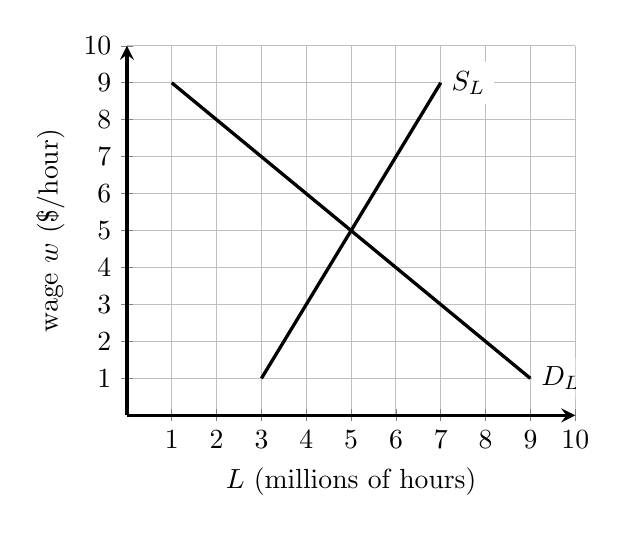
\begin{tikzpicture}
\begin{axis}[
  width={0.6\linewidth},
  grid=both,
  xmin=0,
  xmax=10,
  ymin=0,
  ymax=10,
  xtick={1,2,...,10},
  ytick={1,2,...,10},
  xlabel={$L$ (millions of hours)},
  ylabel={wage $w$ (\$/hour)},
  axis y line=left,
  axis x line=bottom,
  axis line style=very thick
]

\draw[very thick] (axis cs: 3,1)--(axis cs: 7,9) node[right,fill=white]{$S_L$};
\draw[very thick] (axis cs: 1,9)--(axis cs: 9,1) node[right,fill=white]{$D_L$};
\end{axis}
\end{tikzpicture}
\end{center}

\begin{enumerate}
\item Please mark on the graph the market-clearing wage $w^*$ and quantity $L^*$. What is $w^*$ and $L^*$?

\vfill

\clearpage

\item Suppose that employers pay an efficiency wage premium of \$2. That is, they pay \$2 more than the market clearing wage.

\begin{enumerate}

\item Please mark the efficiency wage $\widetilde{w}$. What is $\widetilde{w}$?

\vfill

\item Please mark $\widetilde{L}$ at the quantity of labor actually traded at efficiency wage $\widetilde{w}$. Is it lower or higher than $L^*$?

\vfill

\item Is there a shortage or surplus of labor? How much?

\vfill
\vfill

\end{enumerate}

\item Would you classify unemployment due to efficiency wages as frictional, structural, or cyclical? Why?

\vfill
\vfill

\end{enumerate}

\clearpage

\section{Discouraged workers}

\begin{enumerate}

\item Unemployed workers who are available for a job, and have looked for a job in the last year, but have not looked for a job in the last four weeks because they think they cannot find a job, are classified as \emph{discouraged workers} by the Bureau of Labor Statistics.

Why are these workers not counted as unemployed workers and thus part of the unemployment rate calculation? That is, exactly what criteria do they not meet to be ``unemployed?''

\vfill
\vfill

\item Suppose an economy has 2 million unemployed workers, 1 million discouraged workers, and 10 million employed workers.

\begin{enumerate}

\item What is the unemployment rate (using the standard BLS definitions)?

\vfill

\item If the discouraged workers were included as unemployed, what would the unemployment rate be?

\vfill

\end{enumerate}

\item Does the exclusion of discouraged workers overstate or understate the unemployment rate? 

\vfill
\vfill

\end{enumerate}

\end{document}
